%%%%%%%%%%%%%%%%%%%%%%%%%%%%%%%%%%%%%%%%%%%%%%%%%%%%%%%%%%%%%%%%%%%%%%%%%%%%%%%%%%%%%%%%%%%%%
%									Chapitre 1												%
%%%%%%%%%%%%%%%%%%%%%%%%%%%%%%%%%%%%%%%%%%%%%%%%%%%%%%%%%%%%%%%%%%%%%%%%%%%%%%%%%%%%%%%%%%%%%
\chapter{Etat de l'art}
	\citationChap{
	If I knew how I knew everything I knew, then I would only be able to know half has much, because it will all be clogged up with where I know it from.\\ So I cannot always cite my sources, I'm sorry.
	}{David Mitchell}
	\minitoc
	\newpage

%%%%%%%%%%%%%%%%%%%%%%%%%%%%%%%%%%%%%%%%%%%%%%%%%%%%%%%%%%%%%%%%%%%%%%%%%%%%%%%%%%%%%%%%%%%%%



% Début du chapitre


\section{Contexte}

	Depuis les premiers pas de l'informatique, une question s'est posée : est-ce que les machines peuvent penser ? \cite{turing1950computing} Cette question, bien qu'abstraite dans sa formulation, se réfère à l'intelligence humaine. Il n'est en effet ici pas question de savoir si ce que les ordinateurs font est de la pensée, mais bien si l'on peut reproduire l'intelligence humaine dans un cerveau électronique. Cette question a été le fondement d'un nouveau domaine scientifique qui a été nommé, lors de la conférence de Dartmouth \cite{mccarthy1955proposal} : l'intelligence artificielle (IA).

	Les années qui suivirent n'amenèrent pas de résultat au niveau des attentes des chercheurs. Le domaine était encore trop limité par la puissance de calcul des ordinateurs de cette époque, et les modèles primitifs n'arrivaient qu'à résoudre des tâches simples.

	La première évolution majeure est arrivée dans les années 90, lorsque les processeurs ont dépassé le million de transistors par puce et lorsque les méthodes algorithmiques ont avancé, avec par exemple la recherche rapide dans une base de données. Ces changements ont permis aux modèles d'IA d'exploiter plus de données, plus rapidement et la programmation et les heuristiques étaient les facteurs les plus importants de réussite. Les succès les plus connus de cette époque comptent la victoire de Deep Blue sur Kasparov aux échecs \cite{campbell2002deep}, et le programme Watson d'IBM \cite{ferrucci2012introduction}, qui pourrait être considéré comme le dernier grand projet d'IA de cette période. Il commençait déjà à utiliser quelque chose qui s'est développé en parallèle et qui allait constituer la nouvelle évolution de l'IA : l'apprentissage.

	L'apprentissage automatique est une sous-discipline du domaine de l'IA qui s'est développée tout au long de son histoire et qui est passée sur le devant de la scène depuis les années 2010. C'est une combinaison de plusieurs facteurs qui l'ont amené à dépasser tous les records à ce moment-là : les réseaux de neurones multicouches étaient arrivés à maturation et permettaient l'apprentissage de données avec des représentations à haut niveau d'abstraction. Les dispositifs de calculs devinrent toujours plus puissants, avec notamment les cartes graphiques dédiées devenues programmables et qui permirent d'effectuer du calcul de nombres à virgule flottante en parallèle. Et en dernier, la présence de jeux de données massifs avec lesquels on pouvait entraîner des réseaux toujours plus grands et complexes, et en produisant des résultats toujours plus impressionnants. Les exemples de révolutions applicatives sont légion. La compétition de reconnaissance d'image ImageNet est par exemple passée de taux d'erreurs de 25\% avec des approches classiques à 15\% en 2012 avec le réseau apprenant AlexNet \cite{krizhevsky2012imagenet}, fondé sur des travaux antérieurs de Yann Le Cun \cite{lecun1989backpropagation}. Les années suivantes ont vu l'explosion de ce type de réseaux, qui grâce à leur généricité, ont été appliqués à quasiment tous les domaines de l'informatique et au-delà. En 2017, 5 ans après AlexNet, ImageNet était résolu avec la majorité des participants atteignant des taux d'erreurs inférieurs à 5\%. D'autres succès notables sont la victoire au Go par AlphaGo contre Lee Sedol \cite{silver2016mastering}, et la série de modèles de langage GPT (Generative Pre-trained Transformer) \cite{brown2020language}.

	Malgré ces nombreux succès, des nuages ont commencé à apparaître dans le ciel des réseaux de neurones. GPT-3, le modèle le plus récent d'OpenAI, utilise 175 milliards de paramètres, nécessitant 350 gigaoctets de VRAM juste pour effectuer une inférence. Son coût d'apprentissage a été estimé entre 11 et 28 millions de dollars américains\footnote{https://bdtechtalks.com/2020/09/21/gpt-3-economy-business-model}. La consommation électrique elle, est estimée dans les environs de 190 MWh, correspondant à des émissions en gaz à effet de serre d'un aller-retour terre-lune en voiture\footnote{https://www.theregister.com/2020/11/04/gpt3\_carbon\_footprint\_estimate/}. Le corpus de textes utilisé était 150 fois plus gros que Wikipédia, lui-même inclus dedans. Les performances étaient quant à elles toujours inférieures à un humain, qui lui n'a accès qu'à un cerveau de 25 Watts \cite{kandel2000principles} et un corpus d'apprentissage extrêmement petit en comparaison. On estime qu'un enfant dans une famille aisée entend environ 11,2 millions de mots par an \cite{hart2003early}. Extrapolé pour 20 ans, cela ferait 224 millions de mots pour avoir une bonne maîtrise de la langue, soit 0,05\% des 500 milliards de mots sur lesquels GPT a été entraîné.

	La même observation peut être faite sur tous les succès des réseaux neuronaux. AlphaGo par exemple a eu besoin de 1920 CPUs et 280 GPUs pour battre Lee Sedol, avec une puissance nécessaire estimée à 1 MW\footnote{https://jacquesmattheij.com/another-way-of-looking-at-lee-sedol-vs-alphago/}, soit 100 fois plus que son opposant, Lee Sedol. Les performances surhumaines des réseaux de neurones actuels ne proviennent pas tant de l'intelligence dans les modèles déployés, que de leur capacité à mobiliser de grandes quantités de ressources pour résoudre un problème particulier. Les réseaux de neurones actuels montrant ainsi de plus en plus leurs limites, la question se pose de quelle sera la prochaine épine dorsale de l'IA, et quels seront les développements qui amèneront la prochaine évolution de la discipline. 
	
	Cette thèse s'inscrit dans un courant de pensée qui considère deux approches complémentaires comme étant les clés potentielles vers cette nouvelle évolution : l'accroissement des capacités de calculs par le neuromorphisme et l'augmentation de l'efficacité et de la puissance d'apprentissage par l'émergence et la complexité. Pour mieux situer notre approche, nous allons dans les sections suivantes préciser comment l'inspiration biologique est étroitement liée à la puissance de calcul (\ref{sec:bio}), notamment au travers d'une forme de calcul émergent (\ref{sec:emergence}), qui trouve plus particulièrement un sens dans la vision (\ref{sec:sota:vision}), pour laquelle nos travaux mêlent des principes inspirés des neurosciences (\ref{sec:sota:human_vis}) et de la vision par ordinateur (\ref{sec:sota:computer_vis}).

\subsection{L'inspiration biologique}\label{sec:bio}

	Depuis l'avènement des semi-conducteurs, la puissance computationnelle disponible n'a cessé de s'accroître exponentiellement. La célèbre prophétie auto-réalisatrice de Gordon Moore, que la densité de transistors dans les microprocesseur double tous les deux ans, a fait progresser l'industrie pour lui faire atteindre le million de transistors par puce à l'aube des années 1990, et le milliard en 2006. Au moment de la rédaction de ce manuscrit, la plus grosse puce est le processeur A100 à 54 milliards de transistors\footnote{https://en.wikipedia.org/wiki/Ampere\_(microarchitecture)}.

	Cette progression cache cependant des difficultés pour utiliser efficacement tous ces milliards de transistors. L'architecture de Von Neumann \cite{von1993first} qui sert de modèle depuis les années 50 à quasiment tous les ordinateurs est le point bloquant de la puissance des processeurs. La séparation de la mémoire et du CPU place le bus de données entre les deux comme le centre névralgique de l'ordinateur et sa vitesse est limitée. Ce problème est compensé en partie dans les processeurs modernes avec l'utilisation de cache, mais ce n'est qu'une solution d'appoint qui ne tient pas la mise à l'échelle, car les tailles de cache resteront toujours très inférieures à la mémoire vive. Un second problème, plus important encore, est la limite des performances séquentielles des CPU. 
	
	L'informatique a, dès la machine de Turing, été principalement séquentielle et les algorithmes et processeurs se sont développés pour l'essentiel dans ce paradigme séquentiel. Cela n'a pas posé de problèmes tant que les fréquences augmentaient et que la finesse de gravure se réduisait, amenant toujours plus de performances. Mais un mur de fréquence a été atteint dans les années 2000, dû aux coûts énergétiques et à la chaleur engendrée par les fréquences trop élevées. Depuis les processeurs grand public ont rarement dépassé les 5 Ghz. Cette limite aux performances séquentielles des CPU combinée à la croissance exponentielle du nombre de transistors a naturellement amené vers le développement d'architectures multi-cœurs, qui ont nécessité un développement plus poussé vers le parallélisme tant au niveau matériel qu'algorithmique. C'est ce parallélisme qui a été le catalyseur pour le développement des réseaux de neurones, particulièrement bien parallélisables. La limite de l'architecture de von Neumann elle, reste présente schématiquement. Lors de l'apprentissage d'un réseau de neurones avec de multiples GPU, la mémoire de ceux-ci doit être dupliquée dans chaque carte, et synchronisée régulièrement, si bien que la taille de ces réseaux de neurones est ultimement limitée par la mémoire vive du plus petit GPU. Mais l'architecture de von Neumann n'est pas une fatalité, et il existe de nombreuses idées pour pallier à ses problèmes. La piste que nous avons choisie ici est de s'inspirer de la machine la plus efficace pour traiter de l'information : le cerveau.

	Un cerveau est une machinerie complexe, composé d'environ 170 milliards de cellules chez l'humain, dont la moitié environ sont des neurones, le reste des cellules gliales. C'est un ordre de grandeur similaire au nombre de transistors dans un circuit imprimé récent, mais il existe tout de même des différences importantes entre les deux. Un neurone est capable d'effectuer des opérations beaucoup plus complexes qu'un transistor. Il est également beaucoup plus grand, de l'ordre du micromètre, alors que les transistors ne font que quelques nanomètres. Ce qui explique en partie la différence de taille. Un cerveau humain occupe un volume d'environ 1200 cm\textsuperscript{3}, avec de grandes variations entre les genres et les individus. Les puces informatiques se contentent de deux dimensions et s'étalent sur une petite surface en comparaison, soit 826mm\textsuperscript{2} pour la plus grande. En supposant une épaisseur de 5mm, on obtient un volume de 4,13 cm\textsuperscript{3}. Si l'on compare à volume égal, 1 cm\textsuperscript{3} de cerveau contient environ 140 millions de cellules. Le même centimètre cube de puce informatique peut contenir 13 milliards de transistors, soit un ratio d'une cellule pour 92 transistors. On peut également noter qu'il est possible de réaliser des neurones suivant le modèle \textit{Leaky Integrate and Fire} utilisant moins de 10 transistors \cite{park2021integrate}. Les circuits électroniques ont aussi l'avantage de ne pas être limités en volume comme l'est le cerveau, et l'on peut utiliser une énergie et un volume plus grands de plusieurs ordres de grandeur pour ceux-ci. Ces comparaisons semblent donc indiquer que le nombre de transistors disponibles n'est pas un facteur limitant pour le développement de modèles informatiques plus proches des capacités humaines de raisonnement, puisque l'on pourrait raisonnablement disposer d'une puissance de calcul similaire.

	La différence d'organisation entre un cerveau et un processeur est cependant majeure. Un cerveau fonctionne de façon analogique, évènementielle et asynchrone alors qu'un processeur actuel fonctionne en états discrets (généralement binaires) et synchronisés sur une horloge globale, propre à chaque processeur. Les informations dans le cerveau circulent de façon locale entre neurones voisins et avec très peu de connexions "longue distance". Un processeur est plutôt une chaîne d'assemblage, où toute l'information circule dans un seul sens. La "mémoire vive" dans le cerveau est gérée localement, en modifiant la "chimie neuronale" avec des neurotransmetteurs, en modifiant les connexions synaptiques voire même avec de la neurogenèse. Pour une machine de von Neumann, la mémoire et le calcul sont complètement distincts, et un circuit \textit{Full Adder} fera aussi bien de la cryptographie que du jeu vidéo ou la compilation du code \LaTeX de ce manuscrit. Ces différences sont, de notre point de vue, fondamentales dans ce qui nous sépare des performances et de l'efficacité d'un cerveau humain.

	Récemment, une nouvelle génération de puces appelées "neuromorphiques" a vu le jour chez les fabricants de processeurs. Notamment Loihi\footnote{https://en.wikichip.org/wiki/intel/loihi} d'Intel, ou TrueNorth\footnote{https://www.research.ibm.com/articles/brain-chip.shtml} d'IBM. Ces circuits reprennent des propriétés cérébrales que nous avons évoquées, et comme attendu, la mise à l'échelle de ce genre d'architecture se fait aisément. Intel par exemple le démontre avec ses puces Loihi. Chacune d'entre elles comprend 131 072 neurones, et 10 fois plus de synapses. Une fois combinées par 32 sur une carte \textit{Nahuku} on obtient un système neuromorphique à 4 millions de neurones. Combinez encore ces cartes dans un système plus grand et vous avez \textit{Pohoiki Springs} et ses 100 millions de neurones distribués sur 768 puces. Une question reste cependant ouverte : comment utiliser efficacement toute cette puissance de calcul neuronal ?

\subsection{L'émergence}\label{sec:emergence}

	La première idée pour exploiter efficacement des substrats de calcul neuromorphiques serait de les utiliser avec les outils que nous avons déjà. C'est-à-dire, combiner des algorithmes dans des programmes capables d'effectuer des tâches complexes comme jouer aux échecs, analyser une image ou piloter un avion. Cette approche fonctionne bien pour les ordinateurs classiques, car c'est relativement simple de combiner des algorithmes lorsque les opérations sont séquentielles et la mémoire un ensemble cohérent et interprétable. Il devient plus compliqué de programmer de cette façon des tâches parallèles, car il faut prendre en compte les temporalités de chaque tâche, ce qui ouvre la voie à de nombreux problèmes de blocages, d'incohérences à cause d'interdépendances entre les calculs et augmente significativement le nombre d'erreurs possibles. Le matériel neuromorphique lui est en comparaison proche d'être impossible à programmer car ce que fait chaque neurone dépend non seulement de son état interne, mais aussi du millier de ses neurones voisins et de la temporalité des informations qu'il reçoit. Les chaînes de causalité et de rétroaction sont si complexes et avec de si nombreux éléments que la programmation d'un système neuromorphique à 100 millions de neurones capable de piloter un avion semble hors de portée pour l'intelligence humaine.
	
	Le problème de la complexité n'est cependant pas unique au matériel neuromorphique. Un programmeur moderne n'a pas conscience de l'état de toutes les portes logiques dans un processeur à 50 milliards de transistors lorsqu'il écrit un programme. Mais il arrive à les coordonner pour leur faire simuler le comportement d'un joueur d'échecs ou de go. Cela est permis grâce à des langages de programmation de haut niveau d'abstraction, capables d'effectuer des tâches complexes en restant compréhensibles par un humain. Un tel langage n'existe pas encore pour les puces neuromorphiques. Copier les langages existants qui fonctionnent pour les ordinateurs classiques et les appliquer au neuromorphique copierait également leurs limites, et serait une utilisation inefficace de la puissance de calcul neuronal. Ainsi, il semble nécessaire de trouver des principes fondamentaux pouvant servir de base pour l'élaboration d'un langage de haut niveau qui permettrait d'organiser efficacement le calcul neuromorphique.

	Nous pouvons de nouveau ici nous inspirer de ce que fait la biologie avec le principe d'émergence. L'émergence est un phénomène qui apparaît lorsqu'un ensemble d'éléments a des propriétés différentes de la somme de ses parties. L'émergence peut être observée à tous les niveaux dans la vie. Avec d'un côté les bancs de poissons ou nuées d'oiseaux qui sont le résultat d'un comportement simple au niveau de l'individu : rester proche des autres, aller dans la même direction, etc, et qui amène à une structure plus avancée au niveau du groupe : la nuée. Un phénomène similaire est à l'œuvre chez les fourmis, où par le dépôt de phéromones par chaque fourmi entre la fourmilière et la nourriture, les fourmis empruntent automatiquement le plus court chemin entre les deux. Les phéromones s'évaporant avec le temps, le chemin le plus court sera celui où les phéromones auront le moins de temps pour s'évaporer, et sera de fait la route préférée des fourmis. L'émergence ne se limite cependant pas à l'échelle macroscopique entre individus, mais aussi dans le fonctionnement même d'un organisme.

	Un être humain est composé en masse à 65\% d'oxygène, 19\% de carbone, 10\% d'hydrogène, 3\% d'azote, 2\% de calcium, 1\% de phosphore ainsi que d'autres éléments en plus petites quantités. Cependant, il ne suffit pas de mélanger tous ces éléments ensemble pour qu'un humain apparaisse. Même avec les bonnes molécules cela ne fonctionnerait pas. Pour avoir un humain, il faut que les molécules soient placées au bon endroit les unes par rapport aux autres. C'est à dire, qu'un humain est avant tout une certaine \textit{organisation} de ces molécules. Cette description est valable pour l'ensemble du vivant, jusqu'aux plus petites bactéries et virus. L'étude de l'émergence est donc l'analyse de l'organisation de composants élémentaires pour leur faire adopter des comportements plus complexes. C'est un sujet de recherche pour de nombreux champs scientifiques en plus de la biologie, comme la physique, l'économie et l'informatique avec entre autres, les systèmes complexes.

	Cette idée d'émergence est cruciale dans le fonctionnement du cerveau \cite{turkheimer2019conflicting}, et par conséquent dans l'utilisation efficiente de nos processeurs neuromorphiques. Il n'existe pour l'instant pas de méthode générale qui permette de transformer n'importe quel ensemble de neurones artificiels en système capable de tâches de haut niveau. Nous ne savons pas non plus si une telle méthode générale pourrait exister.

	Il existe des modèles en informatique qui ont pour ambition de faire le lien entre le niveau neuronal et des fonctions plus avancées avec leurs propriétés émergentes et auto-organisatrices. On pourrait considérer le premier pas comme étant l'apprentissage Hebbien. Présenté par Donald Hebb dans son livre \textit{The organisation of behaviour} \cite{hebb1949organisation} et qui introduit l'idée de l'apprentissage associatif, souvent résumé en << \textit{Neurons that fire together, wire together} >>. On peut également citer l'article de Dijkstra sur l'auto-stabilisation \cite{dijkstra1982self}. Le sujet de cette publication est la tolérance aux fautes dans la programmation concurrente. Mais son concept est aussi applicable au domaine de l'émergence où l'on nomme l'auto-stabilisation l'homéostasie. Il s'agit de la capacité d'un système à se maintenir dans un état, comme par exemple la régulation de la température du corps humain. Ce principe d'auto-stabilisation est aussi très présent dans la théorie des champs neuronaux, introduite par \cite{amari1977dynamics}. Les champs neuronaux essayent de définir les dynamiques d'activation dans des populations de neurones à un niveau mathématique. Selon la théorie, les champs neuronaux serait l'élément fondamental pour produire des mécanismes cognitifs complexes \cite{sandamirskaya2014dynamic}. Enfin, nous avons les cartes auto-organisatrices \cite{kohonen-som82}, qui sont un modèle de quantification vectorielle avec la particularité d'organiser automatiquement les neurones pour présenter une forme de continuité spatiale de l'information, de telle sorte que des neurones voisins réagiront à des stimulus similaires.

	Nous avons dans cette thèse utilisé principalement les cartes auto organisatrices (SOM) et les champs neuronaux dynamiques (DNF). Nous les avons choisis parce qu'ils sont très utilisés dans la littérature et appliqués à de nombreux domaines. Leurs capacités à produire des comportements émergents nous intéresse particulièrement, ainsi que leur proximité avec le calcul neuronal qui en fait des modèles décentralisés efficaces pour les systèmes embarqués. Nous avons exploré leur utilisation dans le domaine de la vision et évalué leur adéquation au rôle de couche d'abstraction pour des approches neuromorphiques. Ils seront présentés plus en détail dans les sections suivantes \ref{sec:sota:som} et \ref{sec:sota:dnf}.

\subsection{Particularités de la vision}\label{sec:sota:vision}

	La vision fait partie des sens les plus développés dans la nature ; presque l'intégralité des espèces vertébrées sont dotées d'yeux. Mais en plus d'être très utile, c'est également un sens très complexe. Fondamentalement, il consiste à capter des photons présents dans l'environnement et à en déduire des informations sur celui-ci. Chaque photon arrive dans l'œil ou le capteur avec deux informations : sa longueur d'onde et sa position. En accumulant assez de photons sur un capteur, on peut déduire deux modalités de l'environnement. La luminosité, qui est le nombre de photons provenant d'un endroit particulier et la couleur qui est une combinaison de différentes longueurs d'ondes dans un spectre.

	La vision ne se limite cependant pas à ces propriétés physiques. La lumière, qui est un ensemble de photons, provient d'une source (une ampoule, ou le soleil), et arrive ensuite soit directement, soit après une ou plusieurs réflexions dans l'œil ou le capteur. Ce sont ces réflexions, généralement la première, qui donnent le plus d'informations sur l'environnement. En effet, lorsque de la lumière se reflète sur un objet, il y a une intéraction entre les deux. L'objet absorbe une partie spécifique du spectre lumineux et reflète le reste. La lumière réfléchie contenant dorénavant de l'information sur la position de l'objet et sa couleur. Par conséquent, les informations auquelles nous avons accès grâce à la vision ne sont que partielles. L'objectif du traitement visuel est d'utiliser ces informations partielles pour créer une représentation de l'environnement cohérente.

	Construire une représentation cohérente est cependant complexe. Le premier problème vient de la quantité de données à traiter. De la lumière arrive constamment à nos yeux ou capteurs photosensibles, provenant de l'intégralité du champ visuel. Ce flux continu de données est multiplié par le nombre de pixels ou photorécepteurs. Ceux-ci doivent être en très grand nombre pour couvrir un champ visuel assez large aussi bien horizontalement que verticalement, et pour lesquels une grande densité est nécessaire pour obtenir une précision visuelle suffisante. Par conséquent, le nombre d'informations à analyser par tout système de traitement visuel est conséquent.

	Le second problème vient de la relation des différents pixels ou photorécepteurs entre eux. Un pixel pris isolément ne donne que peu d'informations. Un pixel bleu peut par exemple provenir de la mer, du ciel, d'une voiture, d'un vêtement ou autre. Il est impossible de le savoir juste avec ce pixel, et il faut intégrer les informations contextuelles de voisinages, c'est à dire connaître les valeurs des pixels voisins, voire de l'image entière, pour pouvoir le lier à un objet. Parfois la temporalité est aussi nécessaire pour construire un environnement cohérent. Mais surtout, il faut une connaissance de ce que l'on peut trouver dans des images. Il faut savoir à quoi un objet, un arbre par exemple, correspond matériellement, sa forme physique 3D par exemple, et la rattacher à l'information visuelle qu'elle renvoie, son image, pour construire une représentation cohérente de l'environnement. Cette forme, ou matérialité de l'objet est inaccessible à partir d'une seule image, qui rappelons-le, ne contient que des informations partielles sur la réalité. Une mémoire est donc nécessaire pour tout traitement visuel complexe.

	Tous ces facteurs rendent le traitement visuel un problème particulièrement ardu, qui mobilise un grand nombre de neurones dans le cerveau humain et de gros efforts de recherches en informatique. On oublie facilement cette difficulté car notre système visuel est assez développé pour résoudre aisément ces problèmes de façon inconsciente. La complexité cependant refait surface rapidement lorsque l'on change du format habituel dans lequel sont présentées les images. Différencier des chats et des chiens dans des photographies est facile pour un humain, mais faire la même tâche sur les transformées de fourier de ces photographies est plus compliqué, comme illustré dans la figure \ref{fig:vis:fourier}.

	\begin{figureth}
		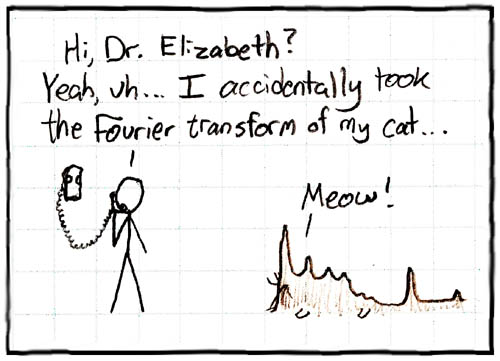
\includegraphics[width=.4\linewidth]{fourier}
		\caption[Illustration de l'efficacité du traitement visuel humain.]{Illustration des capacités du traitement visuel humain. Il est à l'aise pour reconnaître des signatures, même simplifiées, de son environnement visuel habituel mais incapable de reconnaître un chat représenté dans un espace, ici de fourrier, auquel il n'est pas habitué. Si le spectre affiché était effectivement la transformée de Fourier d'un chat.\footnotemark}\label{fig:vis:fourier}
	\end{figureth}

\subsection{Vision humaine}\label{sec:sota:human_vis}

	Cette section a pour but de présenter brièvement et très schématiquement les connaissances actuelles en neurosciences de la vision humaine et de faire le lien avec les modèles que nous avons choisis : les SOM et les DNF. Les informations présentées dans les paragraphes suivants proviennent majoritairement de \cite{gilbert2020constructive}.

	Le système visuel humain commence à la rétine, point de départ du nerf optique pour traverser horizontalement le cerveau jusqu'aux Corps Géniculés Latéraux dans le Thalamus situés à peu près au centre du cerveau, pour finir dans le cortex visuel à l'arrière du cerveau. Les traitements visuels se font tout du long de cette chaîne, avec une gradation allant de traitements de bas niveau dans la rétine, jusqu'aux traitements complexes de haut niveau tel que la reconnaissance de visage dans le cortex visuel. Chaque traitement est fortement parallélisé et se fait dans une zone spécifique du cerveau en première approximation, rendant le système visuel un amalgame de zones spécialisées. La stratégie "diviser pour conquérir" semble donc aussi utilisée dans le cerveau pour traiter des données complexes. Mais il existe aussi de nombreuses connexions entre les zones, chacune influençant des zones voisines et réciproquement.

	Dans les premières couches du cortex visuel (V1, V2, V3 et un peu au delà), les neurones sont organisés en cartes rétinotopiques, c'est à dire en reproduisant l'arrangement spatial de la rétine. Des neurones voisins dans la carte traiterons des zones proches dans le champ visuel. Les DNF sont aussi rétinotopiques (plus de détails dans la section \ref{sec:sota:dnf}). Il y a également une organisation verticale en colonnes de neurones qui partagent des préférences proches comme la position ou l'orientation. C'est un concept qui se rapproche de l'idée qui sous-tend les cartes auto-organisatrices (section \ref{sec:sota:som}). Ainsi l'échange d'information dans le cortex se fait latéralement, verticalement et aussi parfois à longue distance vers une autre zone.

	\footnotetext{Source de l'image : http://xkcd.com/26 reproduit sous licence CC-BY-NC}

	Un autre fait intéressant est que la distribution des neurones qui traitent chaque modalité telle que le contraste, l'orientation ou le mouvement est en proportion équivalente à la distribution de ces modalités dans l'environnement. L'implication est que le système visuel est dépendant de l'environnement. La part de génétique et d'apprentissage dans cette dépendance reste incertaine. Mais elle montre bien qu'une connaissance de l'environnement habituel est utile pour les tâches visuelles.

	Le cortex visuel ne travaille pas de manière isolée du reste du cerveau, et il existe de nombreuses connexions entre celui-ci et des autres aires cérébrales comme le lobe pariétal, qui intègre toutes les informations sensorielles, ou le lobe ventral qui s'occupe de la mémoire et de la reconnaissance d'objets par exemple. Il est estimé qu'environ 10\% de ces connexions entre le système visuel et les autres aires vont dans ce sens, et que les 90\% restants sont dans le sens inverse. Les niveaux supérieurs du cerveau ont donc ainsi une influence importante sur comment les informations visuelles sont traitées à plus bas niveau. La raison de cette disparité est encore inconnue, mais on peut supposer, d'après les observations sur la complexité de la vision évoquées dans la section \ref{sec:sota:vision}, que l'information transmise en sens inverse est à la mesure de la connaissance préalable de l'environnement nécessaire pour compléter l'information partielle de la vision afin de construire une représentation cohérente de l'environnement.

	Un dernier mécanisme essentiel de la vision humaine est l'attention. C'est un mécanisme qui mobilise plusieurs aires cérébrales de différents zones du cerveau. Son intérêt est de concentrer les traitements complexes de la vision à une petite partie seulement du champ visuel. Cela permet d'utiliser moins de ressources pour les traitements complexes, en rendant les stimulus plus simples et en réduisant la surcharge d'informations \cite{evans2011visual}. C'est aussi ce mécanisme qui contrôle en partie les mouvements oculaires pour utiliser efficacement la vision fovéale (une plus grande précision au centre qu'aux bords) des yeux. Nous essayerons de reproduire ce mécanisme avec des DNF dans le chapitre 4. Cependant l'attention humaine utilise une représentation complexe de l'environnement, et d'autres mécanismes cognitifs avancés, et son modèle est toujours un sujet d'études en neurosciences. Nous utiliserons donc une version simplifiée du mécanisme.

\subsection{Détection de nouveauté}\label{sec:sota:computer_vis}

	Il existe de nombreuses fonctions dans la vision et il serait trop ambitieux de vouloir toutes les implémenter dans cette thèse. Ainsi nous avons choisi la détection de nouveauté comme tâche à résoudre. Elle est assez complexe et haut niveau pour ne pas être triviale comme le serait la détection d'orientations (l'angle des lignes d'une image), et nécessite une compréhension de l'environnement pour séparer le fond de la nouveauté. 

	Les domaines de la détection de nouveauté et de la détection de changements sont l'objet de nombreuses recherches et il existe un grand nombre de modèles dans la littérature qui effectuent cette tâche. Nous présenterons les méthodes les plus courantes, celles qui ont les meilleurs résultats et celles qui sont intéressantes pour notre approche.

	Les approches historiques classiques ont généralement consisté à modéliser localement les fonctions de densité de probabilité (\textit{probability density functions} en anglais) pour classifier les pixels du fond et détecter ceux du premier plan. On peut citer par exemple les \textit{Gaussian Mixture Models} (GMM) \cite{zivkovic2004improved}, ou plus récemment \textit{ViBe} \cite{barnich2009vibe}. Certaines travaillent au niveau de groupes de pixels, comme les \textit{Kernel Density Estimators} (KDE) \cite{elgammal2000non}, ou combinent les deux approches \cite{toyama1999wallflower}. Il existe aussi des méthodes différentes, par \textit{Codebook} par exemple, comme dans \cite{kim2004background}. Ces approches classiques ont cependant toutes été supplantées récemment par des modèles fondés sur l'apprentissage.

	Les méthodes les plus performantes actuellement utilisent des réseaux de neurones profonds \cite{tezcan2021bsuv}, \cite{bouwmans2019deep}. L'avantage de ceux-ci est la possibilité d'adapter pour la détection de changements des modèles ayant déjà fait leurs preuves sur d'autres problèmes. L'utilisation de réseaux pré-entraînés permet aussi de réduire le besoin de grands jeux de données d'apprentissages. Les réseaux de neurones profonds étant supervisés par nature, la généralisation requiert cependant un entrainement spécial dû à la variété d'environnements visuels et au peu de données labellisées disponibles.

	Une autre option est de combiner les approches classiques avec des réseaux de neurones, comme par exemple dans \cite{braham2017semantic} qui utilise un modèle neuronal de segmentation sémantique pour mieux représenter les objets détectés, réduisant les erreurs de l'algorithme de détection de changements. \cite{zeng2019combining} combine les résultats de plusieurs algorithmes de détection de changements en les faisant passer par un réseau convolutionnel.

	Il est aussi intéressant de noter que les cartes auto-organisatrices ont déjà été employées pour faire de la détection de nouveauté. Le modèle le plus connu est SOBS (Self-Organized Background Substraction) \cite{maddalena2008self}. Il utilise une petite SOM pour chaque pixel pour apprendre les variations de ce pixel particulier au cours du temps et ainsi décider si la variation fait partie du fond ou si c'est de la nouveauté. Ces petites SOM sont toutes reliées dans un ensemble rétinotopique plus grand représentant le fond complet de l'image et permettant un peu de prendre en compte le voisinage de chaque pixel pour la décision. D'autres versions on été développées plus tard pour améliorer les performances et la robustesse de SOBS \cite{gemignani2016robust}.

	Comme la plupart des approches de détection de nouveauté, nous essayerons d'apprendre un modèle du fond à l'initialisation et de faire la détection de nouveauté en comparant le modèle de fond et l'image courante reçue par la caméra. Nous allons donc apprendre une image avec notre SOM, et utiliser ce que la SOM a appris pour trouver les nouveautés. Nous souhaitons explorer une approche différente de celle de \textit{SOBS}, en ne travaillant pas au niveau des pixels individuels, mais de groupes de pixels. L'idée est de pouvoir intégrer plus d'informations de voisinage dans nos vecteurs d'entrée pour pouvoir effectuer un traitement de plus haut niveau avec les SOM. Nous présenterons ce concept dans le chapitre 2, consacré à la détection de nouveauté. Le chapitre 3 évoquera une amélioration de l'algorithme de la SOM pour en réduire le coût en calculs, car c'est particulièrement important pour une implantation matérielle dans un système embarqué. Le chapitre 4 adjoindra un mécanisme attentionnel avec des DNF à notre détection de nouveauté. 

\newpage
\section{Réseaux neuronaux}

Nous présenterons dans cette partie l'histoire et le fonctionnement des modèles neuronaux que nous avons utilisés. C'est à dire les cartes auto-organisatrices (\ref{sec:sota:som}) et (\ref{sec:sota:som_fc}), les gaz neuronaux en expansion (\ref{sec:sota:gng}) et les champs neuronaux dynamiques (\ref{sec:sota:dnf}).

\subsection{Cartes auto organisatrices}\label{sec:sota:som}

	Les cartes auto-organisatrices regroupent un ensemble de modèles proposé initialement par Teuvo Kohonen \cite{kohonen-som82}. Ces modèles sont caractérisés par leur capacité à projeter des données de façon ordonnée sur un espace d'une dimension plus faible (typiquement une ou deux dimensions). Cette réduction dimensionnelle donne ainsi une "carte" représentative des données qu'on lui a fournies, car les propriétés de voisinage sont conservées. Une des premières utilisations de ces cartes fut la représentation des phonèmes du finnois comme présenté dans la figure \ref{fig:img:phonemes}.

	\begin{figureth}
		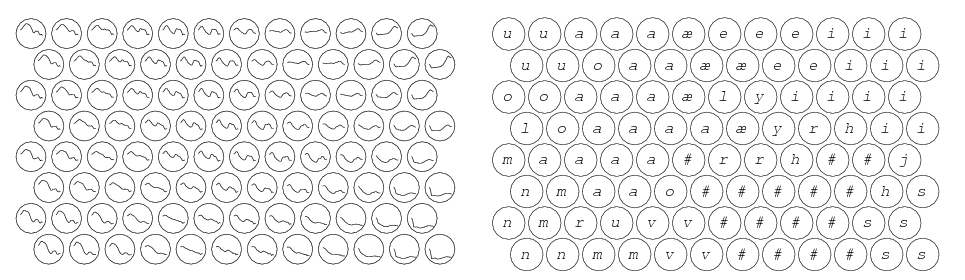
\includegraphics[width=\linewidth]{kohonen_phonemes}
		\caption[Phonème SOM]{Représentation des phonèmes du finnois par la première SOM. A gauche sont représentés les signaux sonores en haute dimension, et à droite leurs phonèmes correspondants. La réduction dimensionnelle provient de l'agencement de ces phonèmes sur la carte. Si ils sont proches entre eux dans leur espace d'entrée (signal), ils seront également proches dans la carte (neurones représentatifs)\footnotemark .}\label{fig:img:phonemes}

	\end{figureth}

	\footnotetext{Source de l'image : http://scholarpedia.org/article/Kohonen\_network licence CC-BY-NC}

	Le but premier de Kohonen était de présenter un modèle capable de représenter informatiquement l'organisation spatiale des informations dans le cortex humain \cite{kohonen-memory}. Il s'inspira pour cela d'un concept du domaine des neurosciences, les colonnes corticales, qui sont des groupes de neurones arrangés verticalement et qui réagissent tous au même stimulus.

	Il y a eu de nombreuses évolutions pendant près de 40 ans d'existence des SOM. En 2002, une bibliographie recensait 5384 articles scientifiques utilisant les SOM \cite{oja2003bibliography}. Ils étaient estimés à plus de 10000 en 2011 \cite{bilbiography-finuni}. Les domaines d'applications sont très variés, allant du traitement du signal de l'analyse d'image et de la parole, jusqu'à la médecine, l'économie, la finance, l'urbanisme et d'autres encore. Pour chacun de ces domaines il y a plusieurs types d'utilisations de la SOM. Elle peut par exemple être utilisée en tant que méthode de visualisation capable de rendre humainement interprétables des données de très grande dimension en les projetant sur des dimensions plus petites. Mais aussi pour faire des traitements sur des données, par exemple pour faire de la classification non supervisée de caractères, de chiffres ou de phonèmes, ou de la détection d'anomalies entre autres. \cite{cottrell2018self} présente une revue récente des différentes approches et applications des SOM. 

\subsection{Principes de fonctionnement}\label{sec:sota:som_fc}
\subsubsection{Préparation des données}

	Nous présentons dans cette section le fonctionnement de l'algorithme de la SOM que nous avons utilisé. Notre version est tout à fait classique et correspond à ce qui est communément utilisé dans la littérature. De très nombreuses variantes existent néanmoins.

	Les données présentées à la SOM doivent être numériques et sous forme de vecteurs. La taille des vecteurs peut être aussi grande que nécessaire, mais toutes les données de la base doivent avoir la même taille de vecteur. Nous n'avons utilisé que des données normalisées, c'est à dire, dont la valeur est comprise entre 0 et 1 inclus. Par exemple pour apprendre des couleurs avec une SOM, on pourra représenter chaque couleur par un vecteur de taille 3, un élément par composante R,G et B par exemple et normalisée pour être comprise entre 0 et 1. L'ordre de présentation des vecteurs lors de l'apprentissage est aléatoire.

\subsubsection{Paramètres}\label{param_som}

	La forme de la SOM dépend de plusieurs paramètres. Le premier est la dimensionnalité. Les SOM peuvent aller d'une dimension de un à un nombre arbitrairement grand. Cependant, en pratique elles ne dépassent que rarement deux dimensions. La raison est que pour la visualisation de données par exemple, pouvoir afficher le résultat complet sur un écran est idéal. C'est aussi la bonne taille pour profiter de la réduction dimensionnelle sans pour autant augmenter de façon exponentielle les coûts en calculs. Une carte de 10 neurones de côté aura 100 neurones en deux dimensions et 1000 en 3 dimensions. Les coûts en calculs étant proportionnels au nombre de neurones, plus de dimensions, avec la même longueur de neurones $n$ implique $n$ fois plus de calculs, où à nombre de neurones équivalents, des cartes plus denses et donc avec moins de réduction dimensionnelle. Nous avons ainsi utilisé exclusivement des cartes bidimensionnelles dans nos expériences. Dans notre cas, nous avons également pris en compte la contrainte matérielle qui rend toutes les dimensions supérieures à deux difficiles à implémenter efficacement en raison des coûts en connexions "longue distance" accrus, car les circuits intégrés sont naturellement en deux dimensions.
	
	Un second paramètre important est ce que nous appelons la topologie de la SOM. Par topologie, nous entendons la forme des connexions entre les neurones qui composent la SOM. Les deux topologies les plus communes pour les SOM sont en grille et hexagonale. Dans la topologie en grille chaque neurone a quatre voisins, un à chaque direction cardinale. En hexagone, chaque neurone a 6 voisins, formant un pavage hexagonal avec les neurones au centre des hexagones (la figure \ref{fig:img:phonemes} est par exemple hexagonale). Ces topologies sont bi-dimensionnelles, mais il est possible de les rendre toriques ou sphériques. Nous n'explorerons pas cette possibilité dans cette thèse, car cela apporte en général plus de contraintes topologiques, c'est plus difficile pour une sphère de bien modéliser l'espace d'entrée que pour une surface plane avec des degrés de libertés au extrémités. D'autres topologies plus exotiques existent et possèdent des propriétés intéressantes \cite{bernard2018np}, cependant nous sommes limités aux topologies classiques, les différences entre les topologies des SOM n'étant pas notre objet d'étude ici.

	Les autres hyper-paramètres de la SOM sont : 
	\begin{itemize}
	\item La taille, communément notée $n$. Elle définit le nombre de neurones par côté de la SOM. Le nombre total de neurones $N$ dans une SOM à deux dimensions est obtenu à partir du carré des côtés : $n^2$. Dans le cas d'une SOM non-carrée, on notera $l$ et $h$ respectivement sa largeur et sa hauteur.
	\item Le nombre d'époques, qui est un entier naturel définissant la durée de l'apprentissage (défini ci-dessous). 
	\item Le coefficient d'apprentissage $\alpha$ (alpha), défini dans $]0,1[$. Il est décroissant linéairement tout au long de l'apprentissage. On notera dans cette thèse la valeur de départ et la valeur finale, toutes les valeurs intermédiaires seront extrapolées par la droite qui coupe ces deux points en fonction de l'époque courante de l'apprentissage. 
	\item Le coefficient de voisinage $\sigma$ (sigma), défini dans $[0,1[$. Il sert à définir l'impact des neurones voisins sur les poids du neurone courant. $\sigma$ est l'écart type du voisinage gaussien d'influence. Ainsi, plus il est élevé, plus la gaussienne sera étalée ce qui amènera à une contrainte topologique plus forte. Inversement, une valeur faible pour ce paramètre produit une gaussienne très centrée et réduit l'influence sur ses voisins de chaque neurone. Si placée à 0, elle enlève toute contrainte topologique et fait que la SOM se comporte comme un k-means. Il est important de noter aussi que nous utilisons une gaussienne normalisée. Cela implique que contrairement à une gaussienne standard, l'intégrale change en fonction de $\sigma$. Ainsi, plus $\sigma$ sera grand, plus l'influence de chaque neurone sera plus grande sur tous les autres, et il n'y a pas de réduction d'influence du fait de l'étalement de la gaussienne. Comme pour le coefficient d'apprentissage, le coefficient de voisinage décroît linéairement pendant l'apprentissage et nous n'indiquerons que les valeurs de départ et de fin. 
	\end{itemize}
	

\subsubsection{Apprentissage}

	Au début de l'apprentissage, tous les poids des neurones sont initialisés aléatoirement entre 0 et 1. L'apprentissage dure un certain nombre d'époques définies avant lancement. Une époque contient le nombre d'itérations requises pour que chaque élément de la base d'apprentissage soit utilisé exactement une seule fois. Lors d'une itération, on sélectionne aléatoirement un vecteur d'apprentissage parmi la base d'apprentissage, qui n'a pas déjà été utilisé lors de cette époque. 

	Une itération se déroule en deux étapes : 
	\begin{itemize}
		\item La phase de recherche, qui consiste à trouver la \textit{Best Matching Unit} (BMU) parmi tous les neurones. Elle correspond au neurone qui a la plus petite distance $L^2$ (distance euclidienne), entre ses poids et le vecteur d'apprentissage.
		\item La phase d'adaptation, qui modifie les poids des neurones selon l'équation suivante :
		\begin{equation}\label{eq:SOM}
			w_i(t+1) = w_i(t)+\alpha(t)\cdot\Theta(\sigma(t),d_{i,bmu})\cdot(v-w_i(t))
		\end{equation} avec $i$ le neurone courant, $w_i$ les poids de ce neurone, $t$ l'itération courante, $\epsilon$ et $\sigma$ des paramètres de la SOM définis dans la section \ref{param_som}. $d_{i, bmu}$ est la distance $L^1$ (distance de manhattan) normalisée entre le neurone $i$ et la BMU pour une SOM en grille. $\Theta$ est une fonction gaussienne centrée normalisée d'écart type $\sigma$. $v$ est le vecteur d'apprentissage.
	\end{itemize}

	On répète ces deux étapes jusqu'à ce que l'on finisse la dernière époque, et l'apprentissage sera terminé. Un exemple d'apprentissage est illustré sur la figure \ref{fig:som_app}

	\begin{figureth}
		\includegraphics[width=.9\linewidth]{unfolding}
		\caption[Apprentissage de SOM]{Apprentissage d'une SOM. Les points bleus sont les vecteurs d'entrée en deux dimensions. Les point rouges les neurones de la SOM et les traits rouges représentent les connexions entre ceux-ci.}\label{fig:som_app}
	\end{figureth}


\subsubsection{Reconstruction}
	
	On appelle reconstruction le fait de remplacer un ensemble de vecteurs, de longueur similaire à ceux sur laquelle la SOM a été apprise, par les vecteurs prototypes des neurones les plus proches.

	Cette reconstruction est par exemple utilisée pour de la compression de données \cite{ettaouil2012improved}, car à la place de mémoriser un ensemble de vecteurs, il n'y a besoin que de mémoriser les vecteurs prototypes de la SOM et l'indice de chaque neurone le plus proche de chaque vecteur d'entrée de l'ensemble. Cette compression est avec perte, du fait que les vecteurs prototypes des neurones ne sont en général pas exactement les mêmes que les vecteurs présentés, même lorsque ceux-ci faisaient partie de la base d'apprentissage.

	\subsection{Gaz Neuronaux en Expansion}\label{sec:sota:gng}

	Bien que nos travaux se soient focalisés sur les cartes auto-organisatrices, notre approche se veut généraliste et transposable à d'autres modèles de quantification vectorielle avec topologie. Nous avons souhaité valider expérimentalement cette transposition en utilisant les Gaz neuronaux en expansion. C'est un autre modèle similaire aux SOM mais avec une approche tout à fait différente sur la topologie, qui devient dynamique et induite par les données d'apprentissage à la place de fixe et prédéterminée comme dans une SOM. 

	\subsubsection{Développements}

	Une évolution majeure inspirée par les cartes auto-organisatrices a été le développement des différents types de gaz neuronaux (Neural Gases, NG), qui a commencé avec \cite{martinetz1991neural}, en tant qu'alternative aux \textit{k-means} car ils ne disposent pas de topologie non plus. Puis ce sont les Gaz Neuronaux en Expansion (Growing Neural Gases, GNG) \cite{fritzke1995growing} qui ont sensiblement amélioré l'approche en ajoutant un mécanisme de croissance qui ajoute des neurones lors de l'apprentissage et une topologie avec des connexions qui se créent et qui disparaissent entre les neurones.

	De nos jours, plusieurs variantes des GNG existent qui améliorent certains aspects de cet algorithme. Notablement, \textit{Growing when required} \cite{marsland2002self} adapte la croissance du nombre de neurones en fonction de ce que le réseau a déjà appris, produisant une forte neurogenèse au début de l'apprentissage et une stabilisation une fois que les données ont été suffisamment apprises. Une autre variante sont les \textit{Icremental growing neural gases} \cite{prudent2005incremental}. Ils permettent d'apprendre de nouvelles données sans oublier les anciennes en combinant plasticité et stabilité.

	Pour la suite, nous avons décidé d'utiliser uniquement l'algorithme des Gaz neuronaux en expansion. C'est le plus utilisé et il est suffisant pour montrer que notre approche est généralisable.

	\subsubsection{Fonctionnement}

	Nous ne présenterons le fonctionnement que des gaz neuronaux en expansion. L'algorithme ne se réduisant pas aisément en quelques formules, nous prendrons une approche itérative, similaire à celle que l'on peut trouver dans l'article original, pour expliquer les différents mécanismes à l'oeuvre. Il est également illustré dans la figure \ref{fig:gng}.

	Une itération se décompose en 9 étapes :
	\begin{enumerate}
		\item Choisir au hasard un élément de la base d'apprentissage parmi ceux qui n'ont pas déjà été tirés lors de cette époque.
		\item Trouver les deux neurones les plus proches : $s_1$ et $s_2$.
		\item Incrémenter l'âge des synapses de tous les voisins directs de $s_1$.
		\item Ajouter la distance euclidienne au carré entre le vecteur d'apprentissage et $s_1$ à la variable d'erreur de $s_1$.
		\item Mettre à jour les poids de $s_1$ et de tous ces voisins directs $s_j$. Les formules sont :
		\begin{equation}
			w_{s_1}(t+1) = w_{s_1}(t) + \epsilon_{\textit{bmu}} \times (v - w_{s_1}(t))
		\end{equation}
		\begin{equation}
			w_{s_j}(t+1) = w_{s_j}(t) + \epsilon_{j} \times (v - w_{s_j}(t))
		\end{equation}
			avec $\epsilon_{\textit{bmu}}$ et $\epsilon_{j}$ des coefficients d'apprentissage.
		\item Enlever toutes les synapses avec un âge supérieur à $a_{\textit{max}}$. Si des neurones se retrouvent sans synapses, les enlever aussi.
		\item Si l'itération courante est un multiple de $\lambda$, insérer un nouveau neurone comme suit :
		\begin{itemize}
			\item Trouver le neurone avec l'erreur la plus élevée $q$.
			\item Créer un nouveau neurone $r$ à distance égale de $q$ et de son voisin direct avec l'erreur la plus élevée $f$.
			\begin{equation}
				w_r(t+1) = \frac{w_q(t) + w_f(t)}{2}  
			\end{equation}
			\item Ajouter des synapses d'âge 0 entre $r$ et $q$ ainsi qu'entre $r$ et $f$. Enlever la synapse entre $q$ et $f$.
			\item Réduire l'erreur de $q$ et $f$ en la multipliant par une constante $\alpha$. Initialiser l'erreur de $r$ avec la nouvelle valeur de l'erreur de $q$.
		\end{itemize}
		\item Réduire toutes les variables d'erreur en les multipliant par une constante $d$.
	\end{enumerate}

	Les hyperparamètres sont donc $\epsilon_{\textit{bmu}}$ et $\epsilon_{j}$ les coefficients d'apprentissage, $a_{\textit{max}}$, l'âge maximum des synapses, $d$ la réduction d'erreur globale et $\alpha$ la réduction lors de l'ajout d'un nouveau neurone. Et enfin le nombre d'époques.

	\begin{figureth}
		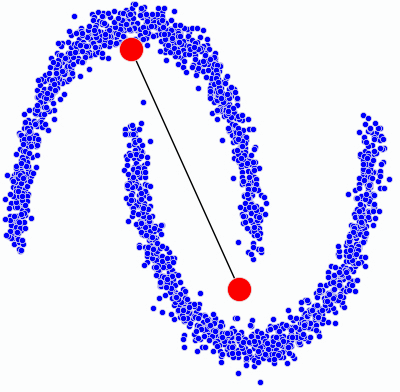
\includegraphics[width=.3\linewidth]{gng_start}
		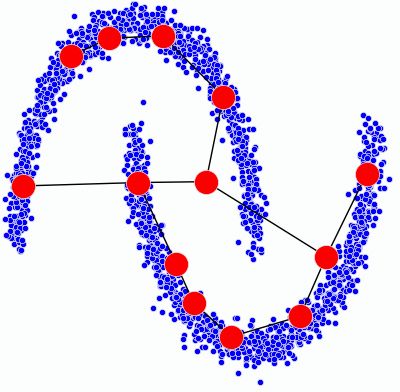
\includegraphics[width=.3\linewidth]{gng_mid}
		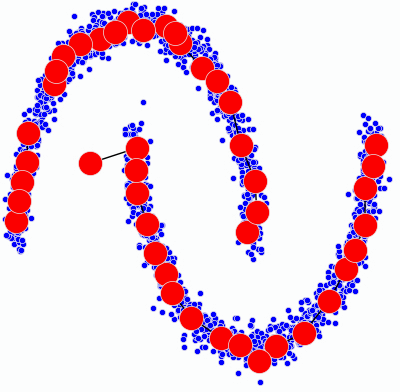
\includegraphics[width=.3\linewidth]{gng_end}
		\caption[Apprentissage de GNG]{Apprentissage d'un GNG de gauche à droite. Les neurones en rouge dans chaque croissant de lune sont connectés entre eux, mais il n'y a pas de connexions entre les neurones des deux croissants de lunes. La topologie du GNG représente la topologie présente dans les données.\footnotemark}\label{fig:gng}
	\end{figureth}

	\footnotetext{Images provenant de https://github.com/AdrienGuille/GrowingNeuralGas, licence MIT}

	L'apprentissage s'arrête au bout d'un certain nombre prédéfini d'époques, comme pour la SOM. L'effet de chaque paramètre peut être compris aisément par le contexte dans lequel il est utilisé, ainsi nous n'irons pas dans le détail de chacun d'entre eux. Le paramètre $\lambda$, ajustant la vitesse de création de nouveaux neurones, sera fixé de telle sorte qu'à la fin de l'apprentissage il y ait le même nombre de neurones dans le GNG que dans la SOM à laquelle on souhaite se comparer. La reconstruction se passe de la même façon que pour la SOM. Les valeurs que l'on aura utilisées pour nos paramètres seront précisées dans la section expérimentale correspondante.

	\subsection{DNF}\label{sec:sota:dnf}

	Les champs neuronaux dynamiques (DNF), introduits par \cite{amari1977dynamics} représentent mathématiquement l'évolution d'une population de neurones. Une dynamique << On center, Off surround >> a été ajoutée par \cite{ellias1975pattern}, qui ont employé des neurones inhibiteurs et excitateurs dans la forme typique de "chapeau mexicain" d'activations (un centre excitateur, un intermédiaire inhibiteur et des bords avec peu d'effet).
	
	Les DNF ont été l'objets de nombreux travaux, notamment dans la vision avec \cite{fix2011dynamic} qui met en œuvre une recherche séquentielle dans un environnement (attention \textit{overt}). Mais aussi pour du suivi de cibles comme par exemple dans \cite{martel2016neuromorphic}.

	Selon leur paramétrage, les DNF peuvent prendre de nombreux rôles. Ils peuvent faire de la sélection, filtrer du bruit ou mémoriser un stimulus grâce à leur adaptabilité et leur mécanisme de \textit{soft winner-takes-all}. C'est pourquoi ils sont étudiés comme modèle de base pour construire des architectures multiDNF et faire émerger des mécanismes cognitifs complexes \cite{sandamirskaya2014dynamic}.

	\subsubsection{Fonctionnement}

	Comme pour les SOM, les DNF peuvent être déclinés en plusieurs dimensions. Nous n'utiliserons que des DNF d'une ou deux dimensions dans cette thèse. Les neurones d'un DNF sont connectés de façon rétinotopique aux entrées, par conséquent, la taille et le nombre de neurones sont définis par la taille de la carte d'entrée. Chaque neurone est également connecté à tous les autres neurones. Enfin, tous les neurones possèdent un potentiel, qui est représenté par un nombre réel. Ce potentiel est noté $u(x,t)$, $x$ étant la position du neurone dans le champ et $t$ un instant de la simulation. La valeur du potentiel d'un neurone intègre les influences des autres neurones, ce qui peut être modélisé sous une forme continue par l'équation différentielle suivante :

	\begin{equation}\label{eq:dnf}
		\tau \frac{\partial u(x, t)}{\partial t} = -u(x,t) + h + \int f(u(x',t))\omega(x-x')\delta x' + S(x,t)g - gi
	\end{equation}

	\begin{equation}\label{eq:diff_gauss}
		\omega(d) = c_{\it exc} \exp \left[ - \frac{d^2}{2 \sigma_{\it exc}^2}\right] - c_{\it inh} \exp \left[ - \frac{d^2}{2 \sigma_{\it inh}^2}\right] 
	\end{equation}

	\begin{equation}
		f(x) = \frac{1}{1+e^{-x}}
	\end{equation}

	\begin{itemize}
    	\item $\tau$ est une constante qui règle la vitesse d'adaptation du DNF.
    	\item $-u(x,t)$ est le terme de fuite. Son rôle est d'inhiber des neurones activés lorsqu'il n'y a plus d'activations par l'entrée ou par d'autres neurones.
		\item $h$ est la valeur de repos du neurone, qui doit être négative.
		\item $f(u(x,t))$ est une fonction logistique. Elle représente l'activation du neurone $x$ au temps $t$. C'est cette valeur qui est généralement utilisée en tant que sortie du DNF.
		\item $\omega(x-x')$ est l'intéraction latérale. Il représente l'effet d'autres neurones sur le potentiel de ce neurone. Nous utilisons une différence de gaussiennes. La gaussienne la plus pointue est excitatrice et la gaussienne plus allongée est inhibitrice. Cela a pour effet que les neurones proches sont excitateurs et les neurones lointains inhibiteurs. On appelle également les neurones ayant un impact excitateur ou inhibiteurs des neurones afférents. La formule est détaillée dans l'équation \ref{eq:diff_gauss}, avec les quatre paramètres associés.
		\item $S(x,t)$ est la valeur au temps $t$ de l'entrée à la position $x$.
		\item $g$ est le gain, et est une constante réelle utilisée pour ajuster l'effet de l'entrée.
		\item $gi$ est l'inhibition globale. C'est une constante divisée par le nombre de neurones présents dans la carte. 

	\end{itemize}

	Par souci de simplicité et de calculabilité, nous avons implémenté une version spatialement et temporellement discrétisée de l'équation \ref{eq:dnf}. Elle est obtenue en manipulant les potentiels d'un ensemble discret de neurones (carte neuronale au lieu de champ neuronal) et en utilisant une simple méthode d'Euler pour estimer l'état de $u(x,t+\Delta t)$ en connaissant $u(x,t)$ :

	\begin{equation}
		u(x, t+\Delta t) = u(x, t) +\frac{\Delta t}{\tau}\left(-u(x, t)+ h + \sum f(u(x', t))\omega(x-x') + S(x, t+\Delta t)g - gi\right)
	\end{equation}

	$\Delta t$ est le pas de temps entre deux estimations, il peut être le même pour tous les neurones (synchrone) ou différent à chaque fois (asynchrone).

	Il est souvent ardu de comprendre le comportement d'un DNF à partir de sa formule mathématique uniquement, ainsi nous préciserons les paramètres et le comportement que nous avons choisis pour chaque DNF utilisé dans le Chapitre 4.

\bibliographystyle{francaissc}
\bibliography{Chapitre1/Biblio}